\chapter{Besluit}
\label{besluit}

	\par Het project heeft een zeer grote omvang en kon tijdens de duurtijd van het projectlab niet volledig voltooid worden. Een overzicht van welke items voltooid werden en welke niet, is weergegeven in figuur \ref{quad_ready}.

	\begin{figure}[H]					  
		  \centering
		  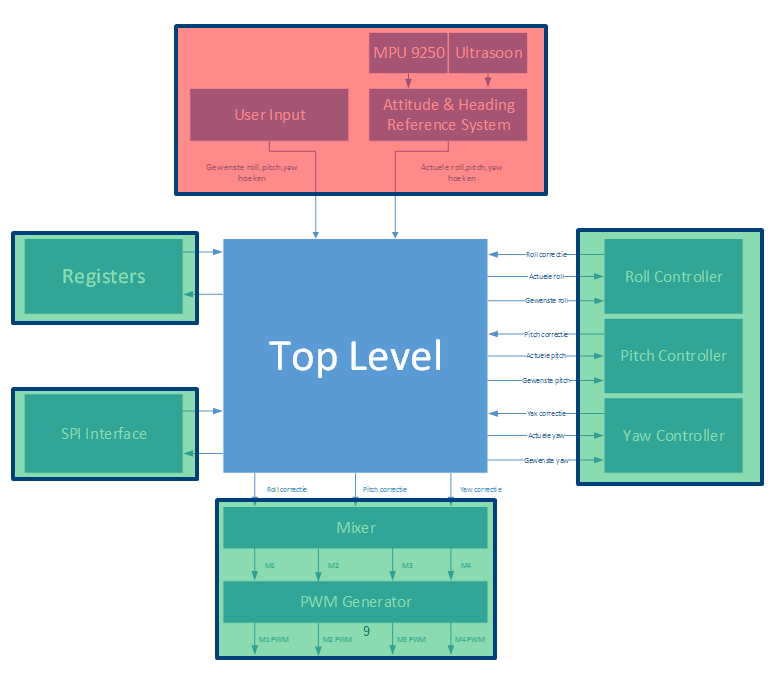
\includegraphics[width=\textwidth]{Besluit/quad_ready.png}
		  \caption{Overzicht van de projectstatus}
		  \label{quad_ready}
	\end{figure}

	\par De PID controller is volledig ge\"implementeerd  en geoptimaliseerd naar resources zodat deze past in de Spartan 6 FPGA. Hierbij werden verschillende iteraties doorlopen die telkens een andere methodiek gebruikten. Aan de hand van Simulink en testbenches werd de werking van de PID controller gevalideerd. De PID controller kon omwille van het ontbreken van sensordata nog niet getest worden op de FPGA zelf. Wel werd al een synthese uitgevoerd om na te gaan of de verschillende PID controllers pasten in het FPGA ontwerp. 

	\par De SPI slave interface werd ontwikkeld aan de hand van dezelfde parameters als het Mojo board gebruikt om te communiceren met de analoge inputs. Op deze manier kan de SPI interface veelzijdig ingezet worden. Via een testbench werd de werking gevalideerd alvorens de interface uit te testen op een FPGA. Wanneer de testbench het gewenste resultaat gaf, werd een test uitgevoerd op de FPGA zelf. Ook hier was de werking perfect en kwamen geen problemen aan het licht.

	\par De PWM generator en motormixer zijn volledig ge\"implementeerd in VHDL. De werking van de PWM generator is reeds getest op een FPGA door het aansturen van de vier verschillende motoren. Hierbij werd ook gebruik gemaakt van de SPI interface om de gewenste PWM instelling te maken. Alles werkt naar behoren. Er dient wel rekening gehouden te worden dat bij het aanleggen van het systeem een vaste PWM waarde aan de motoren wordt aangelegd om deze te activeren. Na ongeveer 1 \'a 2 seconden (beepgeluid bij de motor) zijn de motoren actief en kunnen ze gebruikt worden.

	\par Het quadcopterframe is vollledig geprint, maar dient nog geassambleerd te worden. Door de relatief lange printtijd was er onvoldoende tijd om deze assemblage uit te voeren gedurende het projectlab. De laatste prints waren helaas pas de dag zelf klaar.

	\par Het globale autopilot systeem kon niet getest worden omdat nog niet alle componenten voltooid zijn. De delen die wel getest konden worden, zijn uitvoerig getest en gaven ook het verwachte resultaat.

	\par In het verdere verloop van het project dienen volgende taken nog uitgevoerd te worden.

		\begin{itemize}
			\item Assamblage van het frame.
			\item Alle systeemcomponenten met elkaar verbinden.
			\item Implementeren van AHRS door middel van SPI slave connectie.
			\item Alle data tussen de verschillende componenten in het juiste formaat omzetten.
			\item Bepalen van de K\textsubscript{p}, K\textsubscript{i} en K\textsubscript{d} parameters.
			\item Uitbreiden van de registers.
			\item Globale systeemtest.
		\end{itemize}
